\newcommand{\Versione}{1.0}%Versione Finale
\newcommand{\Data}{2013-01-21}%Data di creazione
%\newcommand{\TipoDocumento}{Relazione finale sullo stage}

\documentclass[a4paper]{article}
\usepackage[utf8x]{inputenc}
\usepackage[italian]{babel}
\usepackage{fancyhdr}
%%pacchetto per il float delle immagini
\usepackage{float}
\usepackage{sidecap,caption}
\usepackage{eurofont}
\usepackage{lastpage}
\usepackage{graphicx}
%\usepackage{fullpage}
\usepackage{setspace}
\usepackage{textcomp}
\usepackage{booktabs}
\usepackage{color}
\usepackage{lscape}
\usepackage{hyperref}
\hypersetup{colorlinks=true, linkcolor=blue, anchorcolor=red, urlcolor=blue}
\usepackage{longtable}
\usepackage{tabularx}
\usepackage{abstract}
\usepackage{appendix}
\usepackage{multicol}
\usepackage{bmpsize}
%%%%%%%%%%%%%%%needed for glossario%%%%%%%%%
%\usepackage{guit}

%\usepackage[acronym]{glossaries}
%\newglossaryentry{parola}{name=parola,description={Si spiega da sé}}
%\newacronym{guit}{\GuIT{}}{Gruppo Utilizzatori Italiani di \TeX{}}
%\addto\captionsitalian{\renewcommand{\glossaryname}{Glossario}}
%\makeglossaries
%%%%%%%%%%%%%%%%%%%%%%%%%fine need glossario
%%%%%%%%%%%glossario prova 2
\usepackage{glossaries}
\addto\captionsitalian{\renewcommand{\glossaryname}{Glossario}}
\newglossaryentry{prova}{name=prova, description={parole a caso}}
\newglossaryentry{dematerializzazione} {name=dematerializzazione, description={processo che ha come obiettivo ultimo la creazione di un flusso di documenti digitali aventi pieno valore giuridico, che vada prima ad affiancare e poi, sul lungo periodo, a sostituire la normale documentazione cartacea presente negli archivi di qualunque attività pubblica o privata.}}
\makeglossaries
%%%%%%%%%%%%%% fine glossario prova 2
\usepackage[all]{hypcap}
\oddsidemargin=.15in
\evensidemargin=.15in
\textwidth=6in
%\topmargin=-.5in
\parindent=0in
%\headheight=1in
\pagestyle{fancy}
\lhead{
\bfseries {\Large \TipoDocumento}\\
\bfseries Versione: \Versione\\
}
\chead{}
\lhead{
%\includegraphics[scale=0.455]{../Logo&Header/SEVENTECH2.png}
}
%\lfoot{\bfseries \TipoDocumento{} v\Versione}
\cfoot{}
\rfoot{\thepage\ of \mypageref{LastPage}}
\newcommand*{\mypageref}[1]{
\hypersetup{linkcolor=black}\pageref{#1}\hypersetup{linkcolor=black}}
%\userpackage{lipsum}
\renewcommand{\footrulewidth}{0.4pt}
%\newcommand{\numref}[1]{\textsl{\nameref{#1} (\ref{#1})}}
%\newcommand{\NomeGruppo}{SevenTech}
%\newcommand{\Progetto}{''3DMob: Grafica 3D su device mobili''}
%\newcommand{\Prop}{Mentis s.r.l.}
%\newcommand{\Glossario}{Al fine di evitare incomprensioni dovute a possibili ambiguità del linguaggio, dei termini e acronimi utilizzati nei documenti, viene allegato il glossario contenuto nel file \emph{Glossario\_{}vX.Y.pdf}.
%Saranno in esso definiti e descritti tutti i termini marcati da una \underline{sottolineatura} nella documentazione fornita.}

%\newcommand{\Prodotto}{

%Il prodotto denominato 3DMob ha lo scopo di fornire un \underline{applicativo} in grado di interpretare \underline{oggetti 3D} a partire dai \underline{formati} \underline{3DS} o \underline{OBJ} e relativo file \underline{MTL}, permettendo all'\underline{utente} di applicare modifiche alla \underline{scena 3D} e di visualizzarne l'anteprima. Il prodotto dovrà successivamente consentire l'\underline{esportazione} del modello 3D nel \underline{formato} \underline{JSON} o \underline{XML}, in modo tale che sia immediatamente compatibile con le \underline{librerie} grafiche \underline{\underline{OpenGL} ES} 2.0, utilizzate nei \underline{device mobili}.
%  Tale formato dovrà essere conforme ai limiti impliciti delle \underline{librerie} grafiche \underline{OpenGL ES} 2.0, in modo che i file esportati possano essere immediatamente utilizzabili nei \underline{device mobili} che supportano tali librerie.

%}
\begin{document}
%\thispagestyle{empty}
%\begin{center}%\centerline{
%\includegraphics[scale=1.05]{../Logo&Header/logo_principale.png}}
%{\href{mailto:grupposwe2013@gmail.com}{\color[rgb]{0.39,0.37,0.38}grupposwe2013@gmail.com}}\\ [3pc]
%{\Huge {3DMob: Grafica 3D su device mobili}}\\[.5pc]
%\underline{\hspace{6in}}\\[3pc]
%{\Huge {\TipoDocumento}}\\[1pc]
%{\emph{Versione \Versione}}\\
%\end{center}
%\vspace{.3in}
\begin{titlepage}
 
\begin{center}
 
% Upper part of the page

\includegraphics[scale=.5]{logoBlack.png}
 
\textsc{\LARGE Università degli Studi di Padova}\\[1.5cm]
 
\textsc{\Large Dipartimento di Matematica\\[0.2cm] Corso di Laurea in Informatica}\\[0.8cm]
  
% Title
\\[0.8cm]{\Huge \doublespacing \bfseries \begin{spacing}{1}{Classificazione firme statiche utilizzando i Hidden~Markov~Models}\end{spacing}}
\\[2cm]

% Author and supervisor
\begin{minipage}{0.4\textwidth}
\begin{flushleft} \large
\emph{Relatore:} \\
Ch.mo Prof. Tullio \textsc{Vardanega}
\end{flushleft}
\end{minipage}
\begin{minipage}{0.4\textwidth}
\begin{flushright} \large
\emph{Laureando:}\\
Alexandru \textsc{Prigoreanu 1004887}
\end{flushright}
\end{minipage}
 
\vfill
 
% Bottom of the page
{\large Anno accademico 2012/2013}
 
\end{center}
 
\end{titlepage}


%\vspace{.4in}

%TESTO DEL SOMMARIO
\null\vspace{2.0in}
\begin{abstract}
La presente relazione ha come scopo la descrizione dell'attività di stage, svolta dal sottoscritto, nel periodo settembre-ottobre 2013 presso l'azienda Corvallis. Il primo capitolo descrive l'azienda ospitante. Il secondo capitolo espone le motivazioni e gli obiettivi del progetto di stage. Il terzo capitolo illustra in modo approfondito le attività effettuate per raggiungere gli obiettivi prefissati. Il quarto ed ultimo capitolo riporta una valutazione a posteriori sul lavoro svolto, sulle conoscenze acquisite e sulla distanza tra le conoscenze richieste e le conoscenze possedute.
\end{abstract}
\vspace{\fill}
%
\newpage



\newpage
\tableofcontents

\newpage

\listoftables
\listoffigures

\newpage

\section{Dominio applicativo}\\
\label{1.0}
La prima parte di questa relazione si prefigge di presentare al lettore il contesto di lavoro dell'azienda ospitante il progetto di stage. Inizialmente descrivo brevemente l'azienda. A seguire effettuo una panoramica sui prodotti e servizi che essa offre e sui clienti che cerca di soddisfare. Infine elenco alcune delle tecnologie di appoggio allo sviluppo software e i processi interni di quest'ultimo.

\subsection{Azienda}
\label{1.1}

\begin{figure}[h!]
\centering

\includegraphics[scale=0.75]{../Logo&Header/logoCorvallis.png}
\caption{ Logo azienda Corvallis}
\end{figure}

Corvallis S.p.A. (http://www.corvallis.it/) è una società italiana presente nel settore dell’Information Technology. Essa applica le sue competenze funzionali, tecnologiche e di processo, acquisite in quasi trenta anni di operatività, in 4 settori strategici per il mondo finance:
\begin{itemize}

\item risparmio gestito e crediti;
\item document management;
\item area compliance;
\item evoluzione tecnologica.\\
\end{itemize}

Corvallis fornisce prodotti e servizi a clienti appartenenti all'ambito finanziario (banche e assicurazioni), industria/servizi e Pubblica Amministrazione. In particolare, Corvallis effettua attività di progettazione e sviluppo software, di fornitura di prodotti software propri e di terzi, di manutenzione e assistenza tecnica, di consulenza.

Il Gruppo Corvallis è composto da più di 600 risorse, tra dipendenti e collaboratori, distribuite in 13 sedi operative nel territorio italiano.

\subsection{Prodotti e clienti}
\label{1.2}
\subsubsection{Banche}
\label{1.2.1}
Corvallis opera da molti anni con i principali istituti di credito e società prodotto. Le aree di competenza sviluppate riguardano:
\begin{itemize}
\item Risparmio Gestito;
\item Finanza;
\item Crediti;
\item Compliance;
\item Governance;
\item Sistemi di Pagamento;
\item Document Management.\\
\end{itemize}
Esempi di prodotti in questo ambito:
\begin{itemize}
\item Antifrode Carte Pagamento, Soluzione per la prevenzione delle frodi sulle carte di pagamento;
\item RG - GeDoFi, Sistema di Gestione Documentale per Banca Depositaria;
\item FIRME - CSIGNgra, Tecnologia di riconoscimento e cattura della firma biometrica.
\end{itemize}
\subsubsection{Assicurazioni}
\label{1.2.2}
Corvallis può effettuare outsourcing nelle compagnie Assicurative per i processi Vita e Danni (IT e backoffice). L'offerta verso le compagnie assicuratrici riguarda le seguenti aree:
\begin{itemize}
\item Sistema Portafoglio Vita e Danni;
\item Sistemi di agenzia;
\item Sistemi sinistri;
\item Compliance;
\item Governance;
\item Servizi di Back Office;
\item Outsourcing;
\item Document Management.
\end{itemize}

\subsubsection{Industria e servizi}
\label{1.2.3}
I clienti di Corvallis sono alcune industrie e imprese appartenenti a differenti settori: Oil~\&~Gas, Engineering, Construction, Aerospace~\&~Defense, Telco, Media. Corvallis possiede competenze anche nell'ambito del Project~\&~Portfolio Management. Inoltre svolge erogazione di servizi di supporto specialistico relativo a prodotti leader di mercato tra i quali Cognos, Qlikview, Hyperion, Business~Object e IrionDQ.
\subsubsection{Pubblica Amministrazione}
\label{1.2.4}
Corvallis offre soluzioni e servizi alle pubbliche amministrazioni. Alcune di queste riguardano:
\begin{itemize}
\item Tributi e fiscalità per gli enti locali;
\item Sistemi informativi territoriali e catastali, GIS, Digital Mapping e cartografia;
\item Document Management;
\item Sistemi Informativi per la catalogazione, conservazione e la tutela dei Beni Culturali.\\
\end{itemize}
Esempi di prodotti in questo ambito:
\begin{itemize}
\item AML - WINTAR, prodotto per la gestione dell'Archivio Unico Informatico
\item AML - Agenzia delle Entrate, prodotto per la gestione delle segnalazioni di vigilanza verso l'Agenzia delle Entrate.
\end{itemize}
\subsection{Tecnologie}
\label{1.3}
Seguono alcune delle tecnologie impiegate nello sviluppo software.

I linguaggi di programmazione più utilizzati sono Java e Cobol.

Il sistema di versionamento in uso è il Concurrent Versions System (CVS).

Alcuni dei database utilizzati sono: DB2, Oracle, MS SQL, PostgreSQL

I framework maggiormente utilizzati sono JBoss e JWolf. JWolf è stato creato dall'azienda stessa.\'{E} un framework per lo sviluppo di applicazioni su tecnologia Java multipiattaforma e multicanale.

L'ambiente di sviluppo per Java è Eclipse.\\

In figura 2 possiamo vedere uno schema riassuntivo di alcune delle tecnologie in uso.
\begin{figure}[h!]
\centering
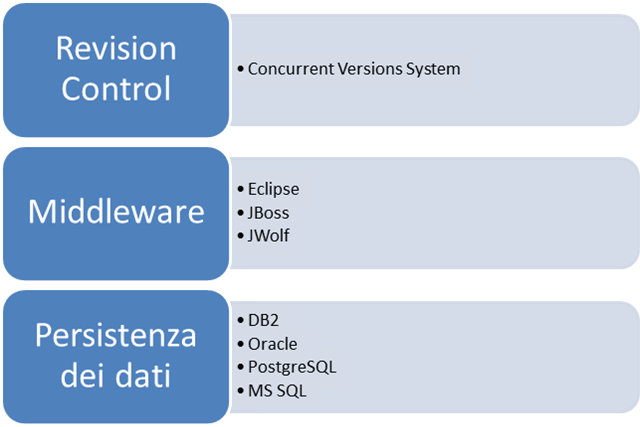
\includegraphics[scale=0.55]{../Logo&Header/tecnologieUsate.png}
\caption{Tecnologie in uso}
\end{figure}


\subsection{Processi interni}
\label{1.4}
Le fasi di sviluppo di un progetto sono costituite da:
\begin{itemize}
\item Coordinamento e Riunioni.
In questa fase vengono pianificate tutte le attività necessarie allo svolgimento del progetto. Gli incontri con i clienti hanno come scopo una efficiente trasmissione di informazioni;
\item Analisi dei requisiti.
L'output dell'attività di analisi è un documento in cui vengono racchiusi tutti i requisiti funzionali, qualitativi, prestazionali e dichiarativi dei quali il prodotto finale dovrà garantirne il soddisfacimento. Il documento serve da input per la fase di progettazione;
\item Progettazione.
Nella fase di progettazione si definiscono le specifiche tecniche delle funzionalità da realizzare. Il risultato di questa fase è il documento di Specifiche Tecniche di Progettazione;
\item Sviluppo.
\'{E} lo stadio esecutivo del progetto con il quale si realizzano i moduli software previsti dal disegno applicativo. In questa fase vengono effettuati test di unità;
\item Test funzionali e di sistema.
I test funzionali hanno lo scopo di verificare che i moduli realizzati durante la fase di codifica rispettino quanto fissato dai requisiti iniziali. Il test di sistema valida il prodotto nella sua interezza;
\item Collaudo con il cliente.
Si tratta di un test di sistema effettuato su un ambiente del cliente e con dati di prova forniti dallo stesso. L'output di questa attività è un verbale che racconta l'esito del collaudo;
\item Documentazione di prodotto.
Questa fase prevede la stesura dei Manuali di Prodotto relativi al software realizzato;\\
\end{itemize}

L'output di ogni fase viene verificato e, se conforme agli standard di qualità dell'azienda, approvato. Altrimenti dovranno essere indicate delle misure correttive per i problemi individuati.\\

In figura 3 vediamo un resoconto delle fasi necessarie allo sviluppo software.
\begin{figure}[h!]
\centering
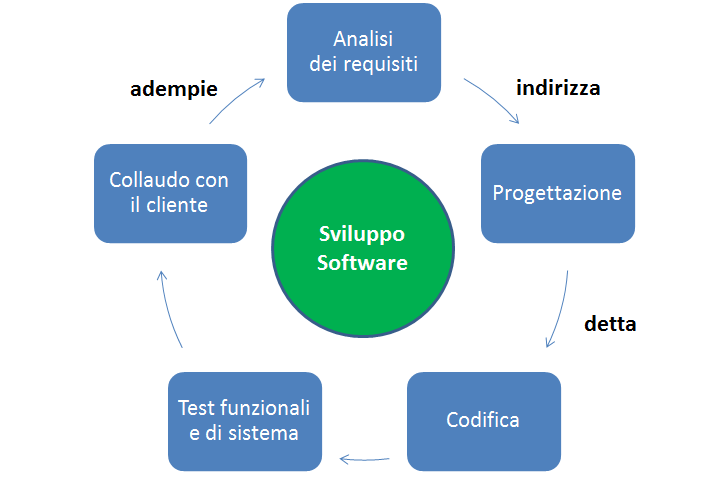
\includegraphics[scale=0.55]{../Logo&Header/sviluppoSoftware.png}
\caption{ Sviluppo Software, ciclo di vita}
\end{figure}

\newpage
\newpage

\section{Progetto aziendale}
\label{2.0}
Questo capitolo ha lo scopo di mostrare al lettore l'ambito in cui si colloca il progetto di stage proposto dall'azienda Corvallis. Inizialmente verranno presentati i motivi che hanno portato alla nascità del progetto. A seguire sarà effettuata una panoramica sulla classificazione delle firme statiche. In seguito verrà descritto il prototipo/classificatore preesistente al progetto di stage. Infine verranno illustrati gli obiettivi, le aspettative e i vincoli del progetto aziendale a cui ho preso parte.\\\\
Visti i notevoli vantaggi in termini di incremento dell'efficienza e di riduzione dei costi che la dematerializzazione garantisce (risparmio relativo ai costi di stampa, acquisto e manutenzione delle stampanti), nell'ambito delle nuove normative alle banche sarà concesso lo scambio di immagini degli assegni bancari. 

In base a questa premessa l'azienda Corvallis ha intuito che il core di un'applicazione bancaria che accetta lo scambio di immagini degli assegni bancari sarà un classificatore di firme statiche accurato, robusto e affidabile. Conseguentemente ha implementato un prototipo per la classificazione delle firme statiche.

\subsection{Introduzione alla classificazione di firme statiche}
\label{2.1}
La firma è un tratto comportamentale di un individuo e costituisce una particolare classe di scrittura dove lettere o parole possono essere non distinguibili. \'{E} considerata un elemento distintivo aventi caratteristiche uniche e personali. 

Nasce quindi la necessità di distinguere tra firme false e firme autentiche.

A seconda del hardware front-end, un sistema di verifica della firma (signature verification system) può essere etichettato come offline o online. Nei sistemi offline la verifica della firma avviene dopo la sottoscrizione della firma. 

- si hanno molte meno informazioni con le firme statiche
- i sistemi online sono di conseguenza più accurati, firma biometrica, pressione, velocità, inclinazione,

Una firma è trattata come un image che conserva un certo pattern di pixel che appartiene a un individuo specifico. I sistemi di verifica delle firme si occupano quindi col esaminare e decidere se una firma appartiene "veramente" al firmatario o no. La verifica di firme è un differente problema dal pattern recognition poiché presi due campioni genuini di un firmatario non sono uguali.

\subsubsection{Prototipo preesistente}
\label{2.1.1}

\subsection{Obiettivi}
\label{2.2}

\subsection{Aspettative}
\label{2.3}

\subsection{Vincoli}
\label{2.4}
\gls{prova}

\newpage

\section{Attività di stage}
\label{3.0}

\subsection{Pianificazione}
\label{3.1}

\subsection{Analisi}
\label{3.2}

\subsubsection{Ricerca di migliorie del prototipo preesistente}
\label{3.2.1}

\subsubsection{Scelta di un nuovo classificatore di firme statiche}
\label{3.2.2}

\subsubsection{Requisiti}
\label{3.2.3}

\subsection{Progettazione}
\label{3.3}

\subsection{Implementazione}
\label{3.4}
\newpage

\section{Valutazione retrospettiva}
\label{4.0}

\subsection{Copertura dei requisiti}
\label{4.1}

\subsubsection{Possibili sviluppi alle attività svolte}
\subsection{Conoscenze acquisite}

\label{4.2}
\subsection{Distanza tra conoscenze richieste e conoscenze possedute}

\label{4.3}
\newpage

%\subsection*{Glossario}
\printglossaries
\addcontentsline{toc}{section}{Glossario}
\label{5.0}

\newpage
\subsection*{Riferimenti}
\addcontentsline{toc}{section}{Riferimenti}
\label{6.0}
\newpage




\end{document}
